\documentclass[tikz,border=8pt]{standalone}
\usepackage[scaled=0.95]{helvet}
\renewcommand{\familydefault}{\sfdefault}
\usetikzlibrary{arrows.meta}
\definecolor{TEJNavy}{HTML}{1E2B55}
\definecolor{TEJBlue}{HTML}{1769AA}
\definecolor{TEJRed}{HTML}{B3261E}
\begin{document}
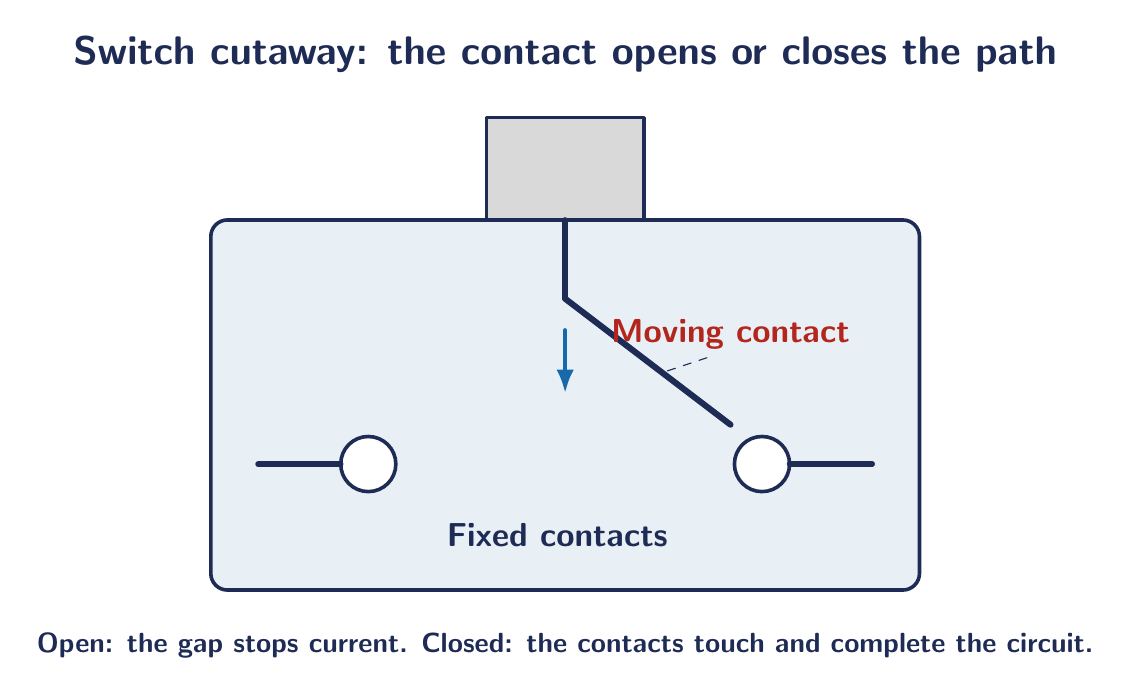
\begin{tikzpicture}[line cap=round,line join=round,font=\sffamily]
  \filldraw[fill=TEJBlue!10,draw=TEJNavy,line width=1.3pt,rounded corners=6pt] (0,0) rectangle (9,4.7);
  \filldraw[fill=black!15,draw=TEJNavy,line width=1.2pt] (3.5,4.7) rectangle (5.5,6.0);
  \draw[TEJNavy,line width=2pt] (4.5,4.7) -- (4.5,3.7);
  \draw[TEJNavy,line width=2.2pt] (4.5,3.7) -- (6.6,2.1);
  \filldraw[fill=white,draw=TEJNavy,line width=1.3pt] (2,1.6) circle (0.35);
  \filldraw[fill=white,draw=TEJNavy,line width=1.3pt] (7,1.6) circle (0.35);
  \draw[TEJNavy,line width=2pt] (0.6,1.6) -- (1.65,1.6);
  \draw[TEJNavy,line width=2pt] (7.35,1.6) -- (8.4,1.6);
  \node[font=\bfseries\Large,text=TEJNavy] at (4.5,6.8) {Switch cutaway: the contact opens or closes the path};
  \node[font=\bfseries\large,text=TEJNavy] at (4.4,0.7) {Fixed contacts};
  \node[font=\bfseries\large,text=TEJRed] at (6.6,3.25) {Moving contact};
  \draw[TEJNavy,dashed] (6.3,2.95) -- (5.7,2.75);
  \draw[-{Latex[length=3mm]},TEJBlue,line width=1.5pt] (4.5,3.3) -- (4.5,2.5);
  \node[font=\bfseries,text=TEJNavy,align=center] at (4.5,-0.7) {Open: the gap stops current. Closed: the contacts touch and complete the circuit.};
\end{tikzpicture}
\end{document}
